\subsection{Stechdorn}

\textbf{Aufbau}
Der Stechdorn hat die Aufgabe, ein Setzloch durch Verdrängung der Topferde auszuheben und anschliessend die fallenden NemaCaps ins Setzloch zu leiten. Dafür wurde auf einen gelochten Stechdorn bewusst verzichtet, da man das Risiko von Verstopfungen nicht eingehen möchte. Mit der realisierten Konstruktion wird dieses Risiko eliminiert. 
\newline
Der Stechdorn besteht aus mehreren Teilen, wobei diese über eine lineare Führung (Punkt 5 in Abbildung \ref{fig:details_stechdorn}) verbunden sind. Dabei wird das Haupt (1) an der Verstellmechanik montiert und macht so die Translation der Setzeinheit mit. Sobald der untere Teil (2, 3) in die Topferde einsticht, fährt die Spitze an den oberen Anschlag der Führung (Detail A). Sobald die Setzeinheit nach oben fährt, öffnet sich die Spitze wieder und das NemaCaps kann durch den Kanal (8) ins ausgehobene Setzloch fallen (Detail B). Dabei soll die Bewegung nur durch die Gewichts- sowie Trägheitskraft der Spitze ausgelöst werden.
\newline
Folgende Überlegungen geben die Lage der linearen Führung vor:
\begin{itemize}
	\item Die lineare Führung soll möglichst parallel zur Bewegungsachse der Setzeinheit verlaufen, sodass möglichst keine Radialkräfte auf den Dorn wirken.
	
	\item Wiederum muss eine seitliche Öffnung der Spitze soweit geschehen, dass die Öffnung (9) frei über dem Setzloch steht (Detail B) und ein freier Fall des NemaCaps möglich ist.
	
	\item Die Verschliessung der Spitze ist in vertikaler Richtung beschränkt durch die Auslegung Spindel. Dabei ist der Abstand C in den Berechnungen mit 15mm angenommen.
\end{itemize}
	\begin{figure}[H]
	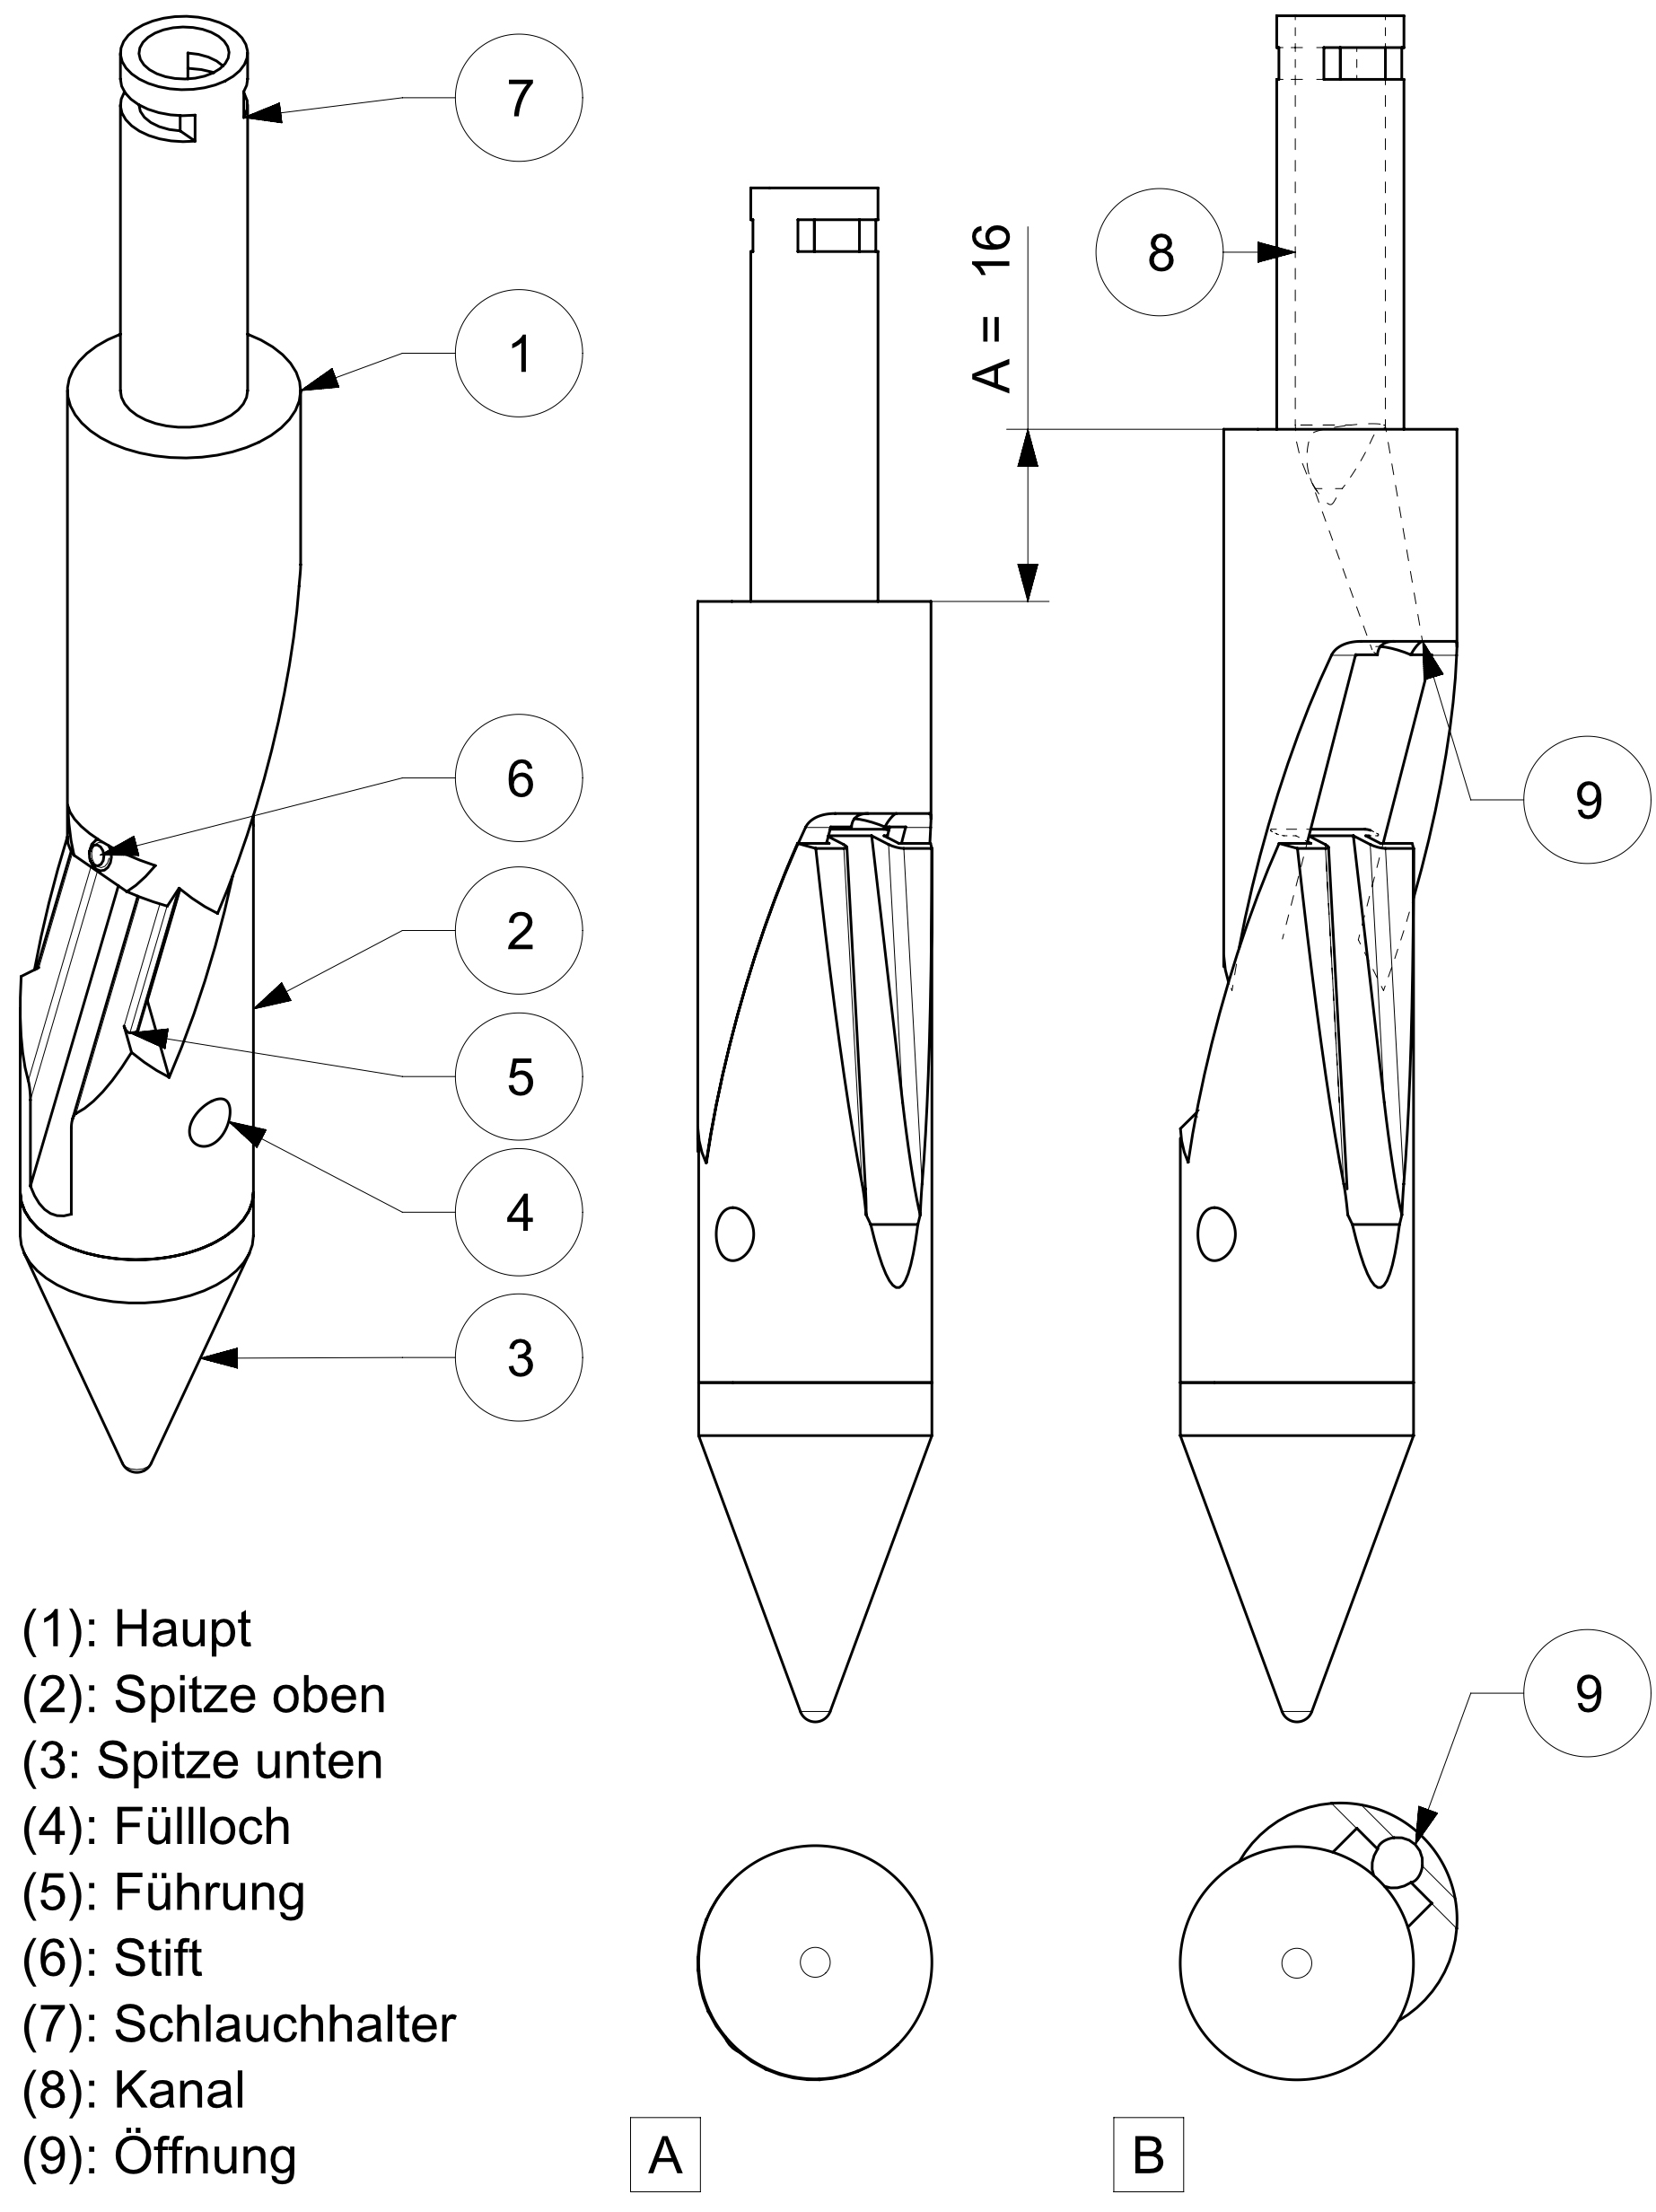
\includegraphics[scale=0.92]{Illustrationen/6-Umsetzung/details_stechdorn.jpg}
	\caption{Übersicht des Stechdorns}
	\label{fig:details_stechdorn}
	\end{figure}


	\begin{figure}[H]
	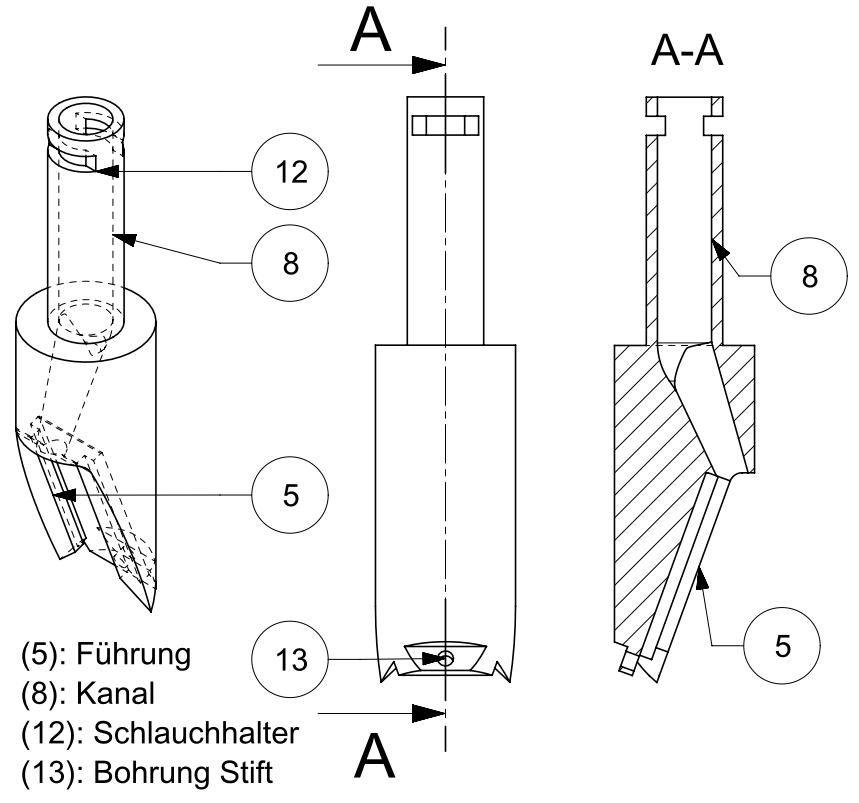
\includegraphics[scale=0.62]{Illustrationen/6-Umsetzung/details_haupt.PNG}
	\caption{Details zum Haupt}
	\label{fig:details_haupt}
	\end{figure}

	\begin{figure}[H]
	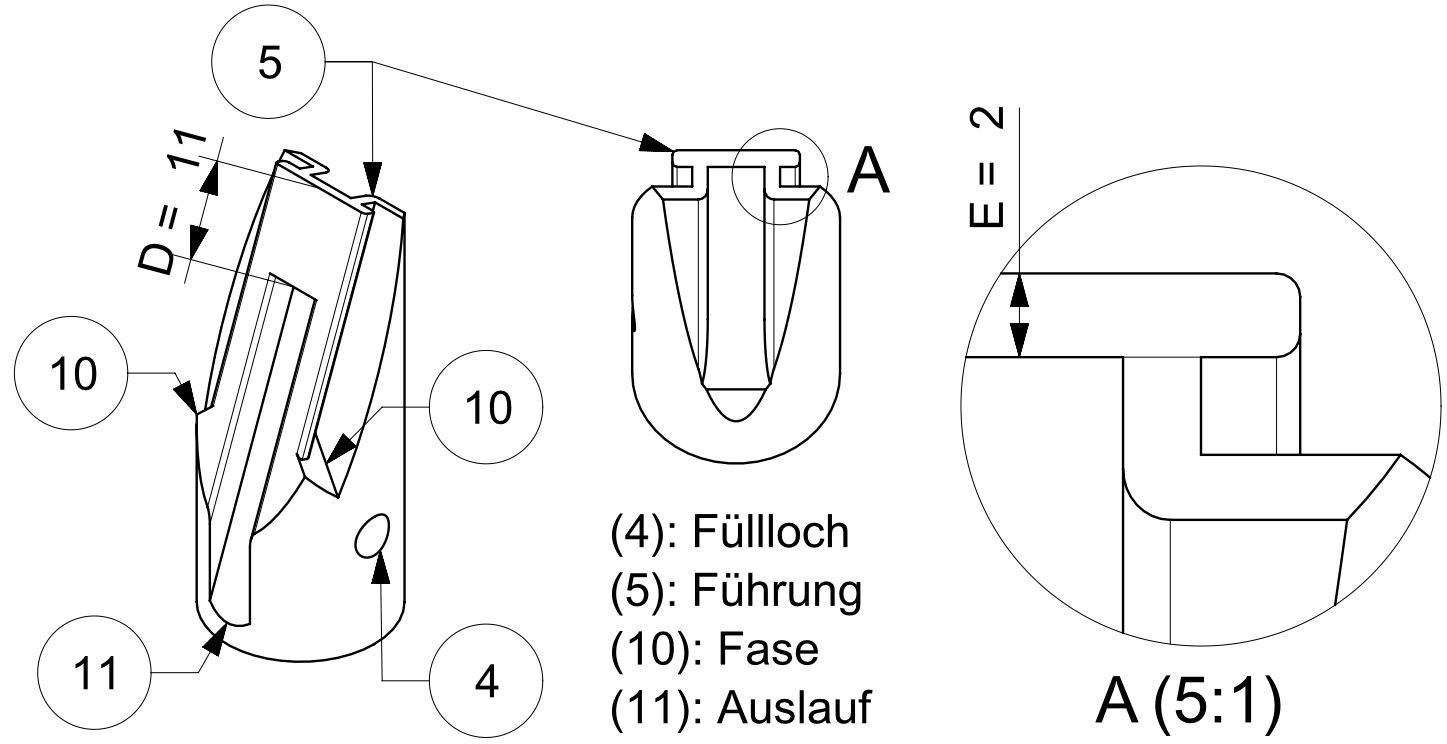
\includegraphics[scale=0.42]{Illustrationen/6-Umsetzung/details_spitze_oben.PNG}
	\caption{Details Spitze oben}
	\label{fig:details_spitze_oben}
	\end{figure}

\textbf{Funktion}